\section{Experimental methods}
A brief overview of the employed experimental techniques are presented here. Mole fraction time histories of methane ($\mathrm{CH_4}$), acetylene ($\mathrm{C_2H_2}$), and ethylene ($\mathrm{C_2H_4}$) were captured using CW laser absorption at 3.365 $\mu$m, 2.998 $\mu$m, and 10.532 $\mu$m, respectively~\citep{stranic2014laser,pinkowski2019multi, cassady2020thermal}. CB volume fraction was measured using laser light extinction at $\lambda$=633~nm and 1064~nm.% with absorption function E(m) of 0.174 and 0.203~\citep{lee1981optical}, respectively. 
Additionally, soot samples were collected onto imaging stubs mounted in the shock-tube endwall. A schematic of the experimental setup for laser diagnostics in the shock tube is shown in Fig.\ref{fig:laserlayout}. Samples were extracted from the interior surface of the shock tube endwall after each experiment to allow for imaging and analysis of the particulates. TEM images were recorded with a FEI Tecnai G2 F20 X-TWIN microscope and Gatan SC200 camera for all test cases.


\begin{figure}[!t]
	\centering
	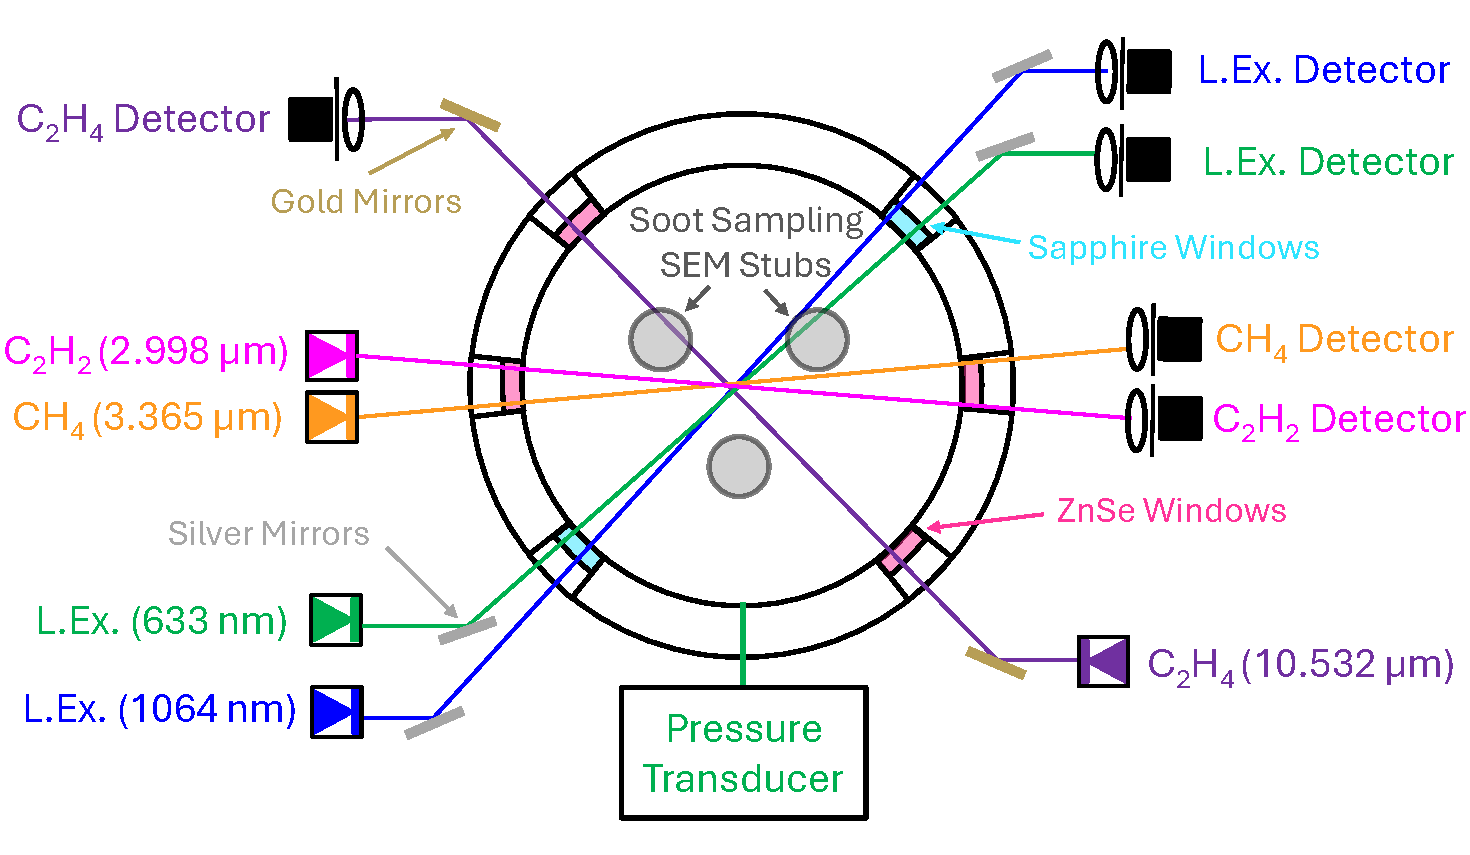
\includegraphics[width=0.48\textwidth]{Figures/laser_setup.pdf}
	\caption{Layout of the laser diagnostics and shock-tube setup. Spatial and spectral filtering is employed to ensure high-quality absorbance measurements to infer species mole fractions and soot volume fraction. Soot samples are collected at the shock-tube endwall. All lasers are aligned in a plane 1 cm from the endwall}
	\label{fig:laserlayout} 
\end{figure}